\documentclass{sciposter}
\usepackage{natbib}
\usepackage[colorlinks=true, citecolor=blue, urlcolor=blue, linkcolor=blue]{hyperref}
\bibliographystyle{alpha}
\usepackage{amsmath}
\usepackage{amssymb}
\usepackage{multicol}
\usepackage{graphicx,url}
\usepackage[spanish]{babel}
\usepackage[utf8]{inputenc}
\usepackage[T1]{fontenc}
\usepackage{mathpazo}
\usepackage{caption}
\usepackage[most]{tcolorbox}
\usepackage{comment}
\renewcommand{\familydefault}{\rmdefault}
\newtheorem{Def}{Definición}

\definecolor{BoxCol}{rgb}{0.0, 0.2, 0.5}
\definecolor{SectionCol}{rgb}{255, 255, 255}

\newtcolorbox{defbox}[1]{
  colback=BoxCol!5,
  colframe=BoxCol,
  fonttitle=\bfseries,
  coltitle=white,
  title=#1
}
% ---------------------------------------------------------------
% ENCABEZADO PERSONALIZADO
% Fila superior: escudo izquierdo -- banner oficial (centrado) -- escudo derecho
% Debajo: título y autores.
% Reemplaza los nombres de archivo por tus imágenes reales.
% ---------------------------------------------------------------
\renewcommand{\maketitle}{%
  \noindent
  \begin{minipage}[c]{0.22\textwidth}
    \centering
    \vspace{-3cm}
    
\includegraphics[width=0.4\linewidth]{assets/main/escudo-unal.jpg}\hfill
    \hspace{-0.2cm}
\includegraphics[width=0.53\linewidth]{assets/main/escudo-puj.jpg.png}
  \end{minipage}%
  \begin{minipage}[c]{0.56\textwidth}
    \centering
    \vspace{-3cm}
    
\includegraphics[width=0.95\linewidth]{assets/main/Encabezado_Poster_ALTENCOA11_2026.png}
  \end{minipage}%
  \begin{minipage}[c]{0.22\textwidth}
    \centering
    \vspace{-3cm}
    \includegraphics[width=0.65\linewidth]{POSTER_CURVAS_DEL_DRAGON/assets/main/Qr-repositorio.png}\\[0.2cm]
    {\vspace{-0.5cm}\small\bfseries Repositorio del proyecto\\}
    %{\small\bfseries Código para generar las curvas}
  \end{minipage}%
  \vspace{-0.6cm}
  \begin{center}
    {\Huge\bfseries Curvas del Dragón revisitadas}\\[0.4cm]
    {\Large Juan Esteban Huertas Serrano$^1$, Alejandro Manrique Roca$^2$}\\
    $^1$Universidad Nacional de Colombia, Bogotá - Colombia. juanestebanhu@gmail.com \\ 
    $^2$Pontificia Universidad Javeriana, Bogotá - Colombia. alejandro.manrike.roca@gmail.com
  \end{center}  
  \vspace{0.4cm}
  \hrule
  \vspace{0.3cm}
}
\begin{document}
\conference{{\bf ALTENCOA11 - 2026}, San Juan de Pasto, 9 al 11 de octubre}
\maketitle
\begin{multicols*}{3}
\section{Introducción}
En 1966, los físicos John Heighway y William Harter se preguntaron acerca del patrón generado al plegar repetidamente una hoja de papel por la mitad, siempre en el mismo sentido \cite{davis1970}. Notaron que la secuencia de pliegues que se formaba al desdoblar la hoja seguía un comportamiento autosimilar. Sin embargo, la imposibilidad física de doblar un papel numerosas veces hizo necesarias ideas matemáticas que modelaran tal comportamiento de forma abstracta. Esto dio origen al dragón de Heighway y a la familia de curvas fractales generadas bajo la idea del \textit{plegado de papel} \cite{gamboa2020}, denominadas curvas del dragón. %En el presente póster se presentan la definición y las principales propiedades del dragón de Heighway y las curvas del dragón \cite{davis1970, gamboa2020}, y se revisitan desde la perspectiva categórica introducida por Tom Leinster en \cite{Lei11} para el estudio de sistemas autosimilares.%
\vspace{-0.5cm}
%%%%%%%%%%%%%%%%%%%%%%%%%%%%%%%%%%%%%%%%%%%%%%%
\section{Palabra del Dragón}
%Para formalizar el patrón de los pliegues, es posible codificar la secuencia de giros sobre un alfabeto binario \cite{davis1970}.
\begin{center}
    \includegraphics[width=1\linewidth]{POSTER_CURVAS_DEL_DRAGON/assets/main/plegado-imagen.jpeg}
\end{center}
\begin{defbox}{Definición.}
Considere el conjunto de palabras sobre el alfabeto binario $\Sigma = \{U, D\}$, dotado de la operación concatenación. Para una palabra $w$, denotamos por $\overline{w^R}$ la palabra que resulta de invertir el orden de $w$ e intercambiar las $U$ por $D$ entre sí. La \textbf{palabra del dragón} $S_n$ se define como:
\vspace{0.25cm}
\begin{enumerate}
\item $S_0 = \lambda$ es la palabra vacía. 
\item $S_1 = D$.
\item Recursivamente, $S_{n+1} = S_n D \overline{(S_n)^R}$.
\end{enumerate}



\end{defbox}
La palabra $S_{n+1}$ contiene a $S_n$, seguida de una $D$ que representa un nuevo doblez, y finalmente a $S_n$ invertida, como sucede con la secuencia de dobleces al plegar el papel.
\begin{defbox}{Ejemplo.}
\begin{enumerate}
    \item $S_1 = D$
    \item $S_2 = DDU$
    \item $S_3 = DDUDDUU$
    \item $S_4 = DDUDDUUDDDUUDUU$
\end{enumerate}
\end{defbox}
%Es posible definir la palabra del dragón $S_n$ de una manera equivalente, como indica la siguiente proposición.
\begin{defbox}{Proposición. (Construcción por intercalación)}
Dada la palabra $S_n = a_1 a_2 \cdots a_m$ de longitud $m = 2^n - 1$. Entonces la palabra $S_{n+1}$ se obtiene insertando alternadamente los símbolos $D$ y $U$ entre las letras de $S_n$:
\begin{center}
$S_{n+1} = D\, a_1 \, U \, a_2 \, D \, a_3 \, U \, \dots \, D \, a_m \, U$.
\end{center}
\end{defbox}
Note que cada letra de $S_n$ permanece fija en todas las palabras posteriores, lo permite definir la \textbf{palabra infinita del dragón} como el \textit{límite de la sucesión} de palabras 
\begin{center}
$S_\infty : = \mathsf{lim}_{n \to \infty}S_n$
\end{center}
\[ = 
\underset{\substack{\uparrow\\[1pt]S_1}}{{D}} 
\, {D} \, 
\underset{\substack{\uparrow\\[1pt]S_2}}{{U}} 
\, {D} \, {D} \, {U} \, 
\underset{\substack{\uparrow\\[1pt]S_3}}{{U}} 
\, {D} \, {D} \, {D} \, {U} \, {U} \, {D} \, {U} \, 
\underset{\substack{\uparrow\\[1pt]S_4}}{U}\dots
\]

Esta sucesión de símbolos codifica los giros de la curva del dragón que se obtienen al desdoblar por completo el papel.
\begin{comment}
\[
S_\infty = 
\textcolor{blue}{\underrightarrow{%
  \strut \textcolor{orange}{\underrightarrow{%
    \strut \textcolor{blue}{\underrightarrow{\strut \mathbf{D}}_{S_1}} 
    \, \textcolor{orange}{\mathbf{D \, U}}%
  }_{S_2}} 
  \, \textcolor{blue}{\text{D \, D \, U \, U}}%
}_{S_3}} \; \dots
\]
\end{comment}
\vspace{-1cm}
\section{De la palabra a la curva}
Para pasar de la palabra $S_n$ a una curva en el plano complejo, se traza un segmento inicial de $0$ a $1$, y luego se recorre cada letra de la palabra $S_n$: cada $U$ indica un giro de $90^\circ$ en sentido antihorario y cada $D$ un giro de $90^\circ$ en sentido horario, tras lo cual se traza un segmento unitario en dicha dirección. Este proceso se repite hasta agotar todas las letras de $S_n$. Equivalentemente, es posible identificar cada vértice de la curva con un punto $z_k \in \mathbb{C}$ definido como sigue: tome $z_0 = 0$ y considere
\begin{center}
$\delta(s) = \begin{cases} +1 & \text{si } s = D \\ -1 & \text{si } s = U \end{cases}, \qquad \theta_k = \sum_{j=1}^{k} \delta(a_j)$.
\end{center}
La orientación del $k$-ésimo segmento es $i^{\theta_{k-1}}$, y la posición final tras $n$ segmentos está dada por
\begin{center}
$z_n = \sum_{k=0}^{n-1} i^{\theta_k}$.
\end{center}
Con tal definición, la curva poligonal $\theta _m =(z_0, z_1, \cdots , z_m)$ hace el recorrido del dragón de Heighway.
\begin{center}
\fcolorbox{gray!30}{white}{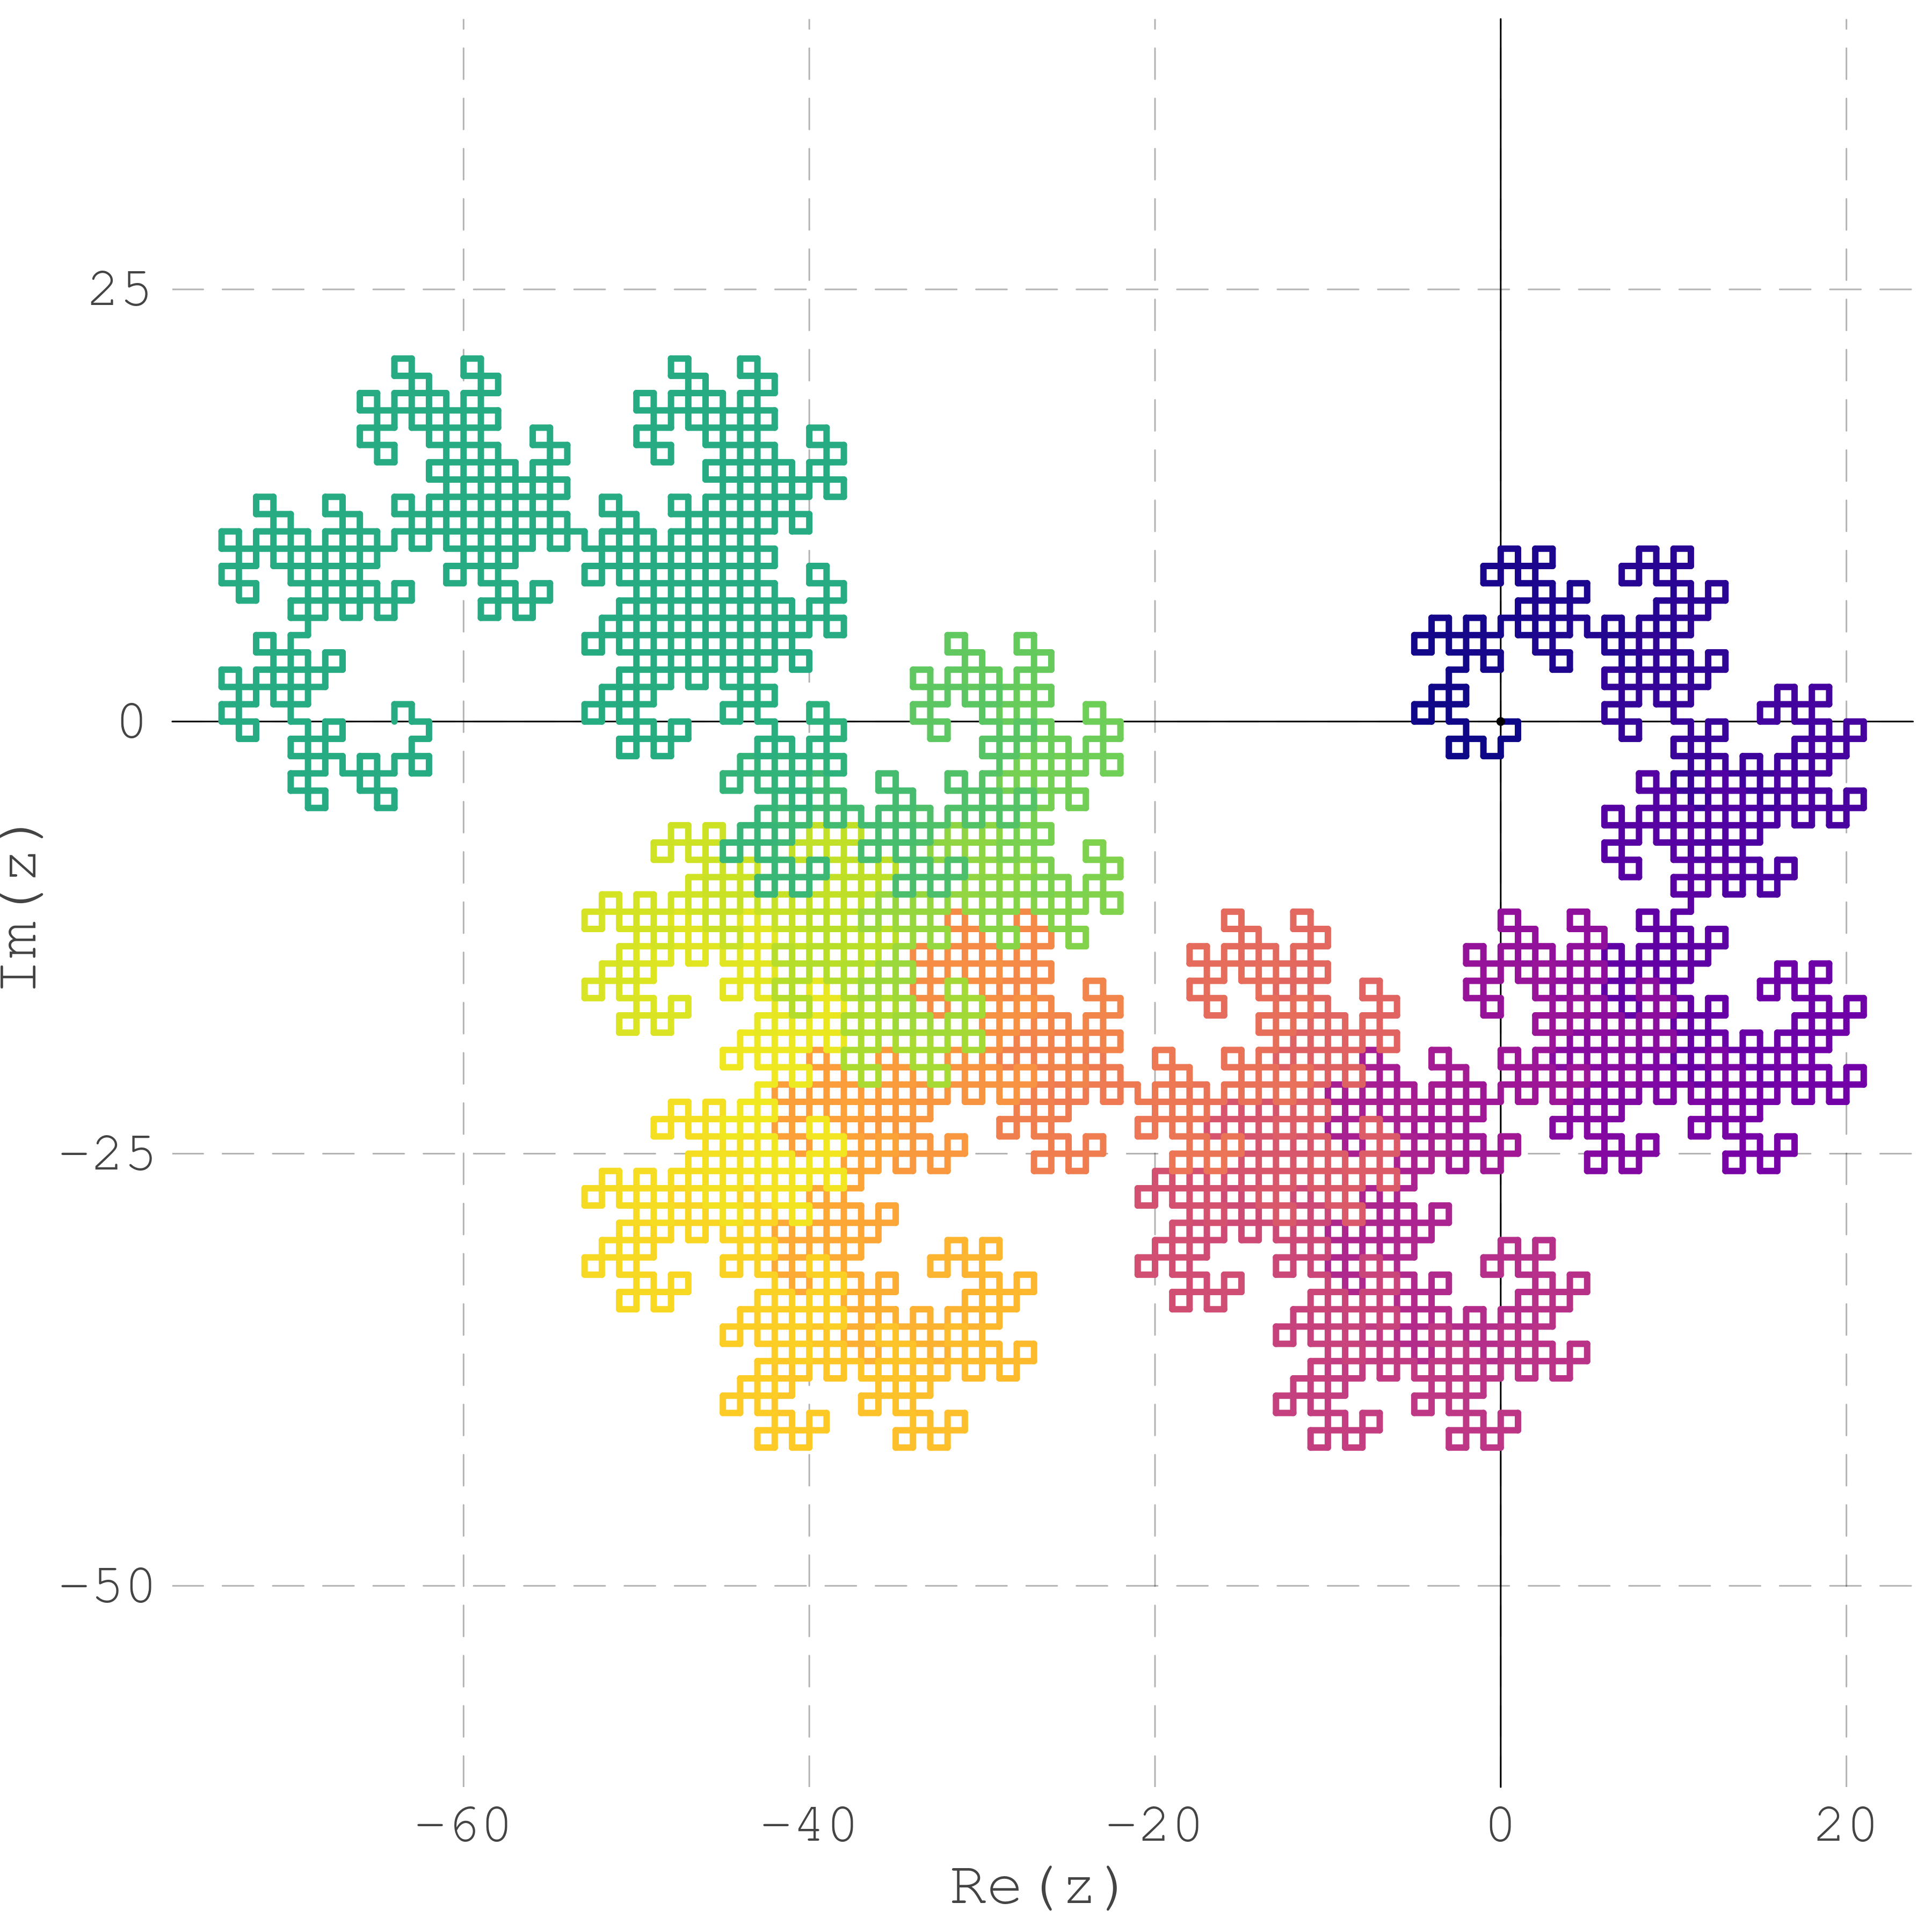
\includegraphics[width=\dimexpr\linewidth-2\fboxsep-2\fboxrule\relax]{assets/main/curva_dragon_ejes.png}}
\captionof{figure}{Representación de la curva del dragón.}
\end{center}
\vspace{-0.8cm}
%%%%%%%%%%%%%%%%%%%%%%%%%%%%%%
\section{Propiedades}
\begin{defbox}{Proposición. (No autointersección)}
La curva poligonal $\theta_n$ definida previamente es inyectiva salvo, posiblemente, en un conjunto finito de vértices donde puede tocarse a sí misma. Sin embargo, sus aristas nunca se cruzan interiormente.
\end{defbox}
\begin{defbox}{Observación. (Semillas generadoras)}
Definimos la \textbf{semilla generadora} como $S_1$. Al cambiar tal semilla por otra palabra y definir $S_{n+1}=S_n S_{1} \overline{(S_n)^R}$, podemos llegar a distintas curvas como las siguientes:
\begin{center}
    \setlength{\fboxsep}{1pt} % Grosor del espacio interno del marco
    \setlength{\fboxrule}{0.5pt} % Grosor de la línea del marco
    
    % Primera fila
    \fcolorbox{gray!40}{white}{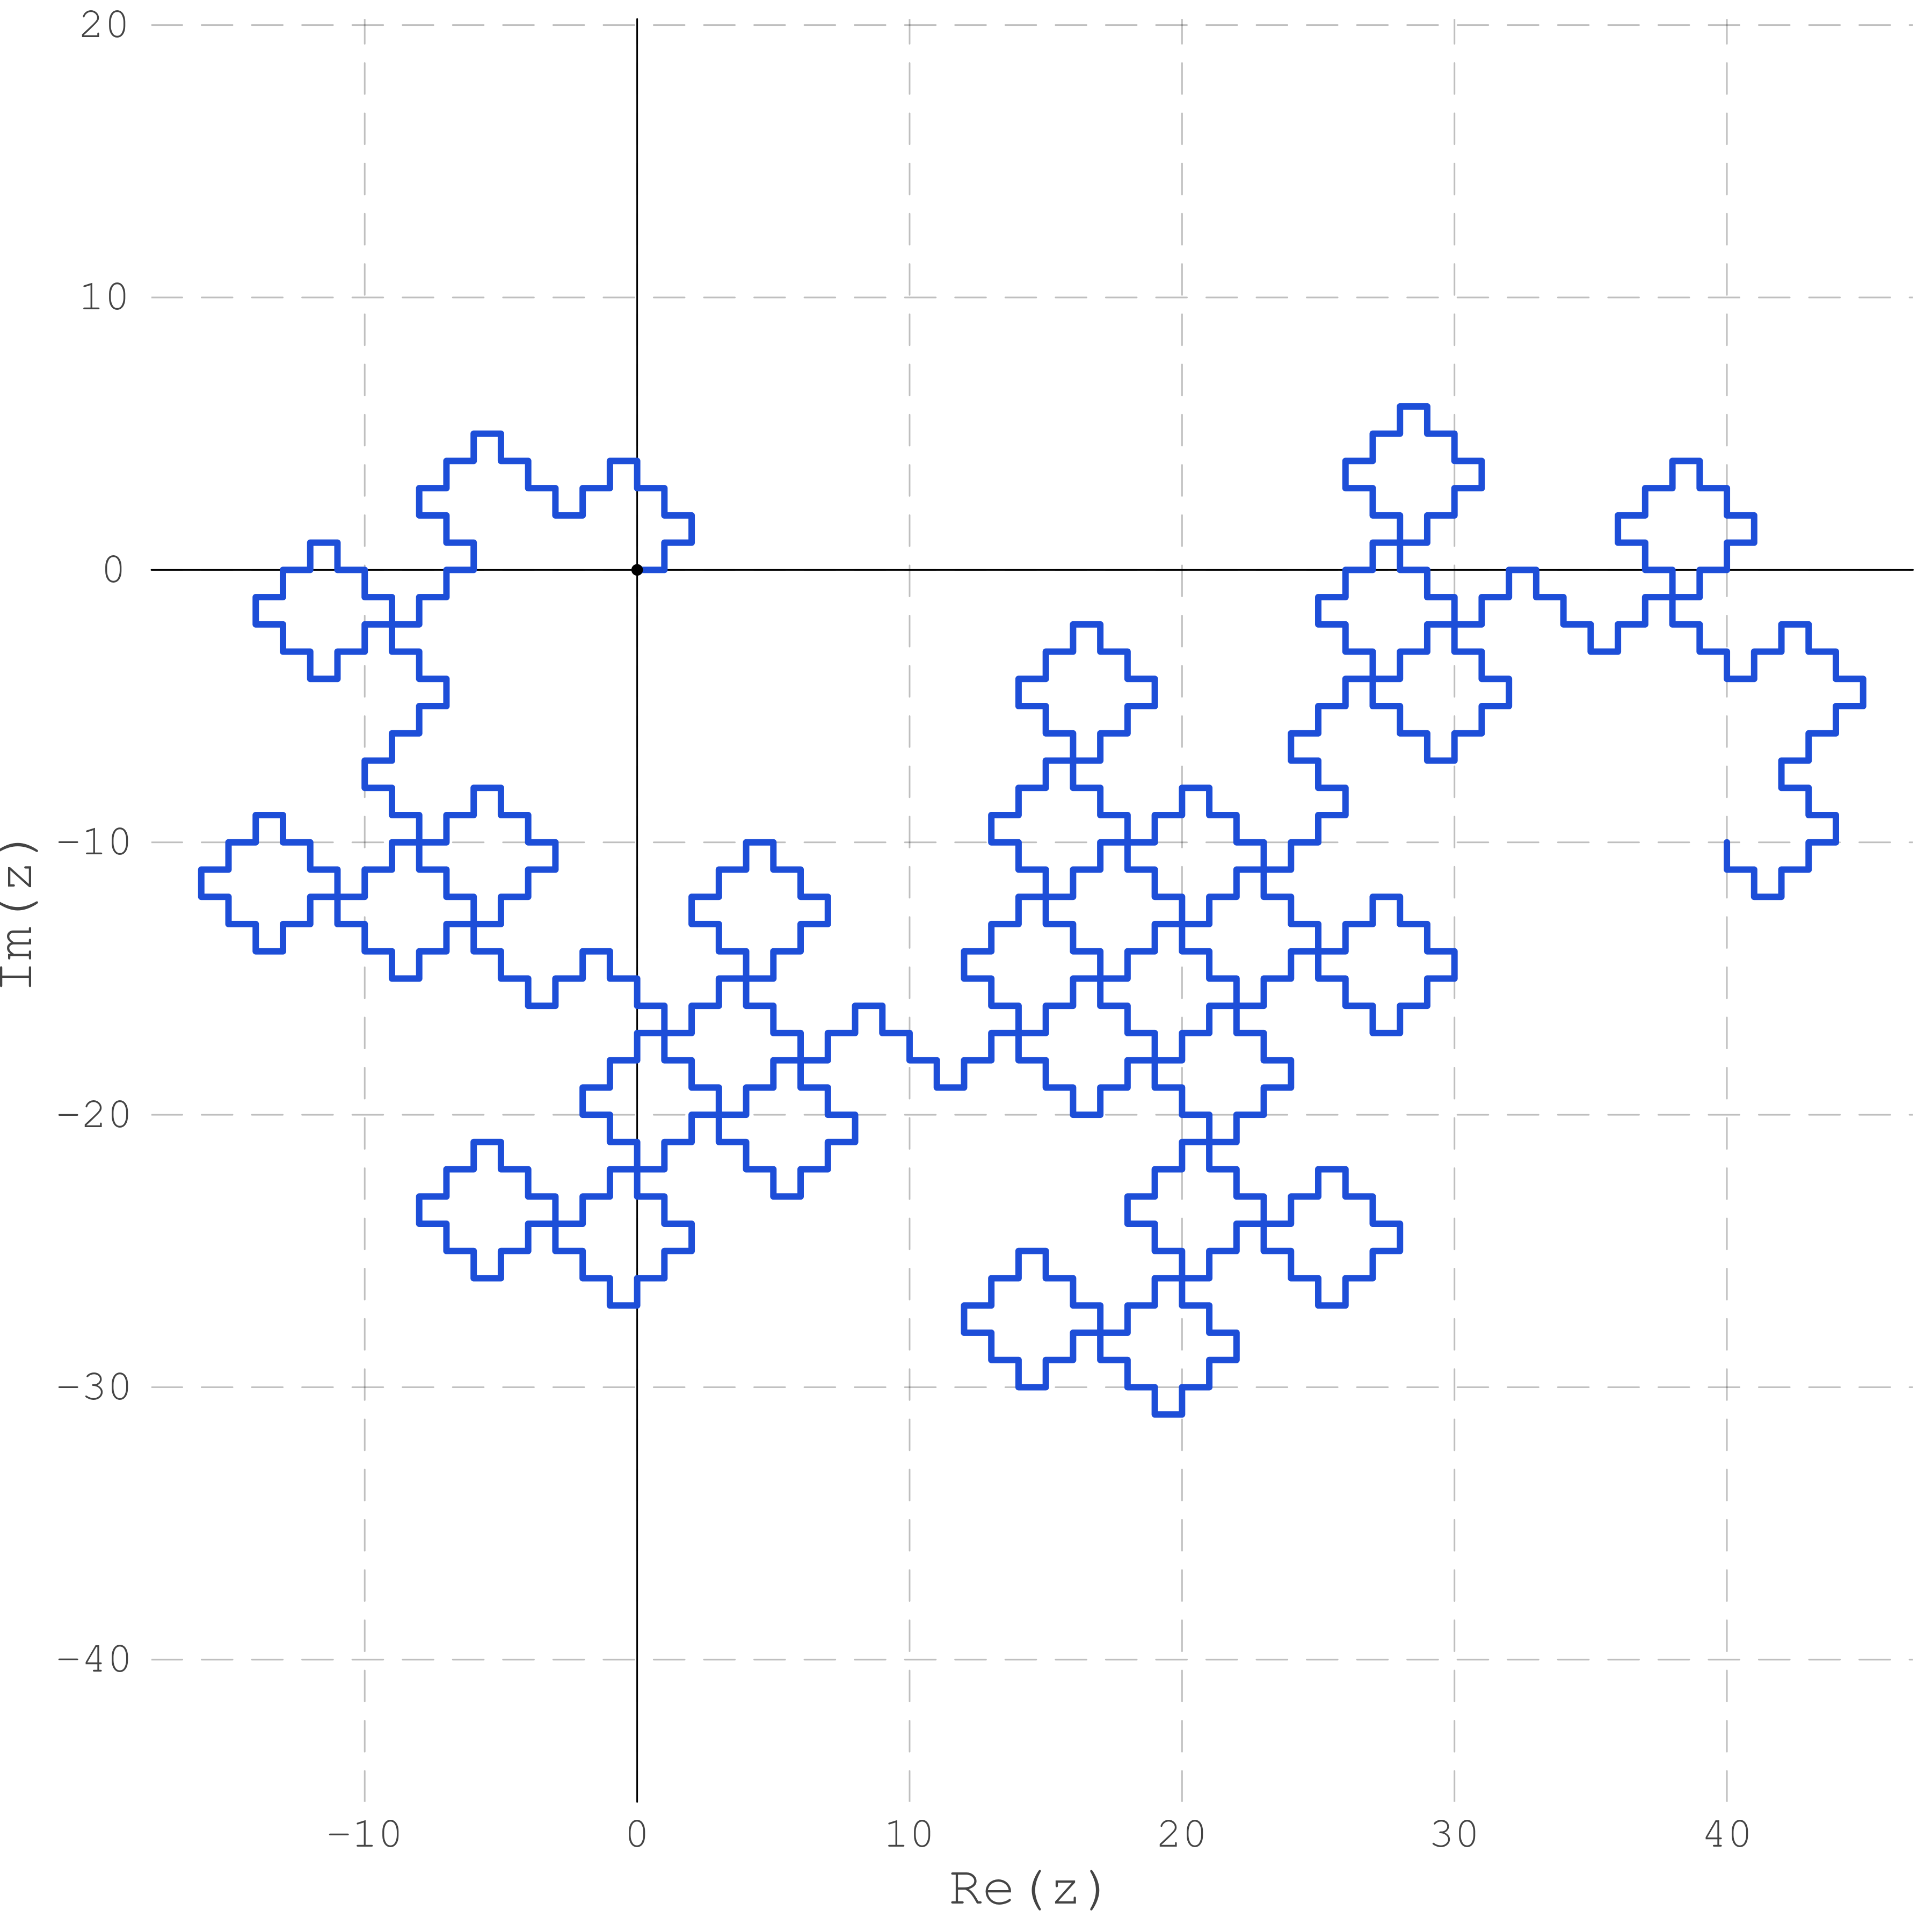
\includegraphics[width=0.46\linewidth]{assets/seed/curva_dragon_DUDDU_i7_p3.png}}\hspace{0.2cm}%
    \fcolorbox{gray!40}{white}{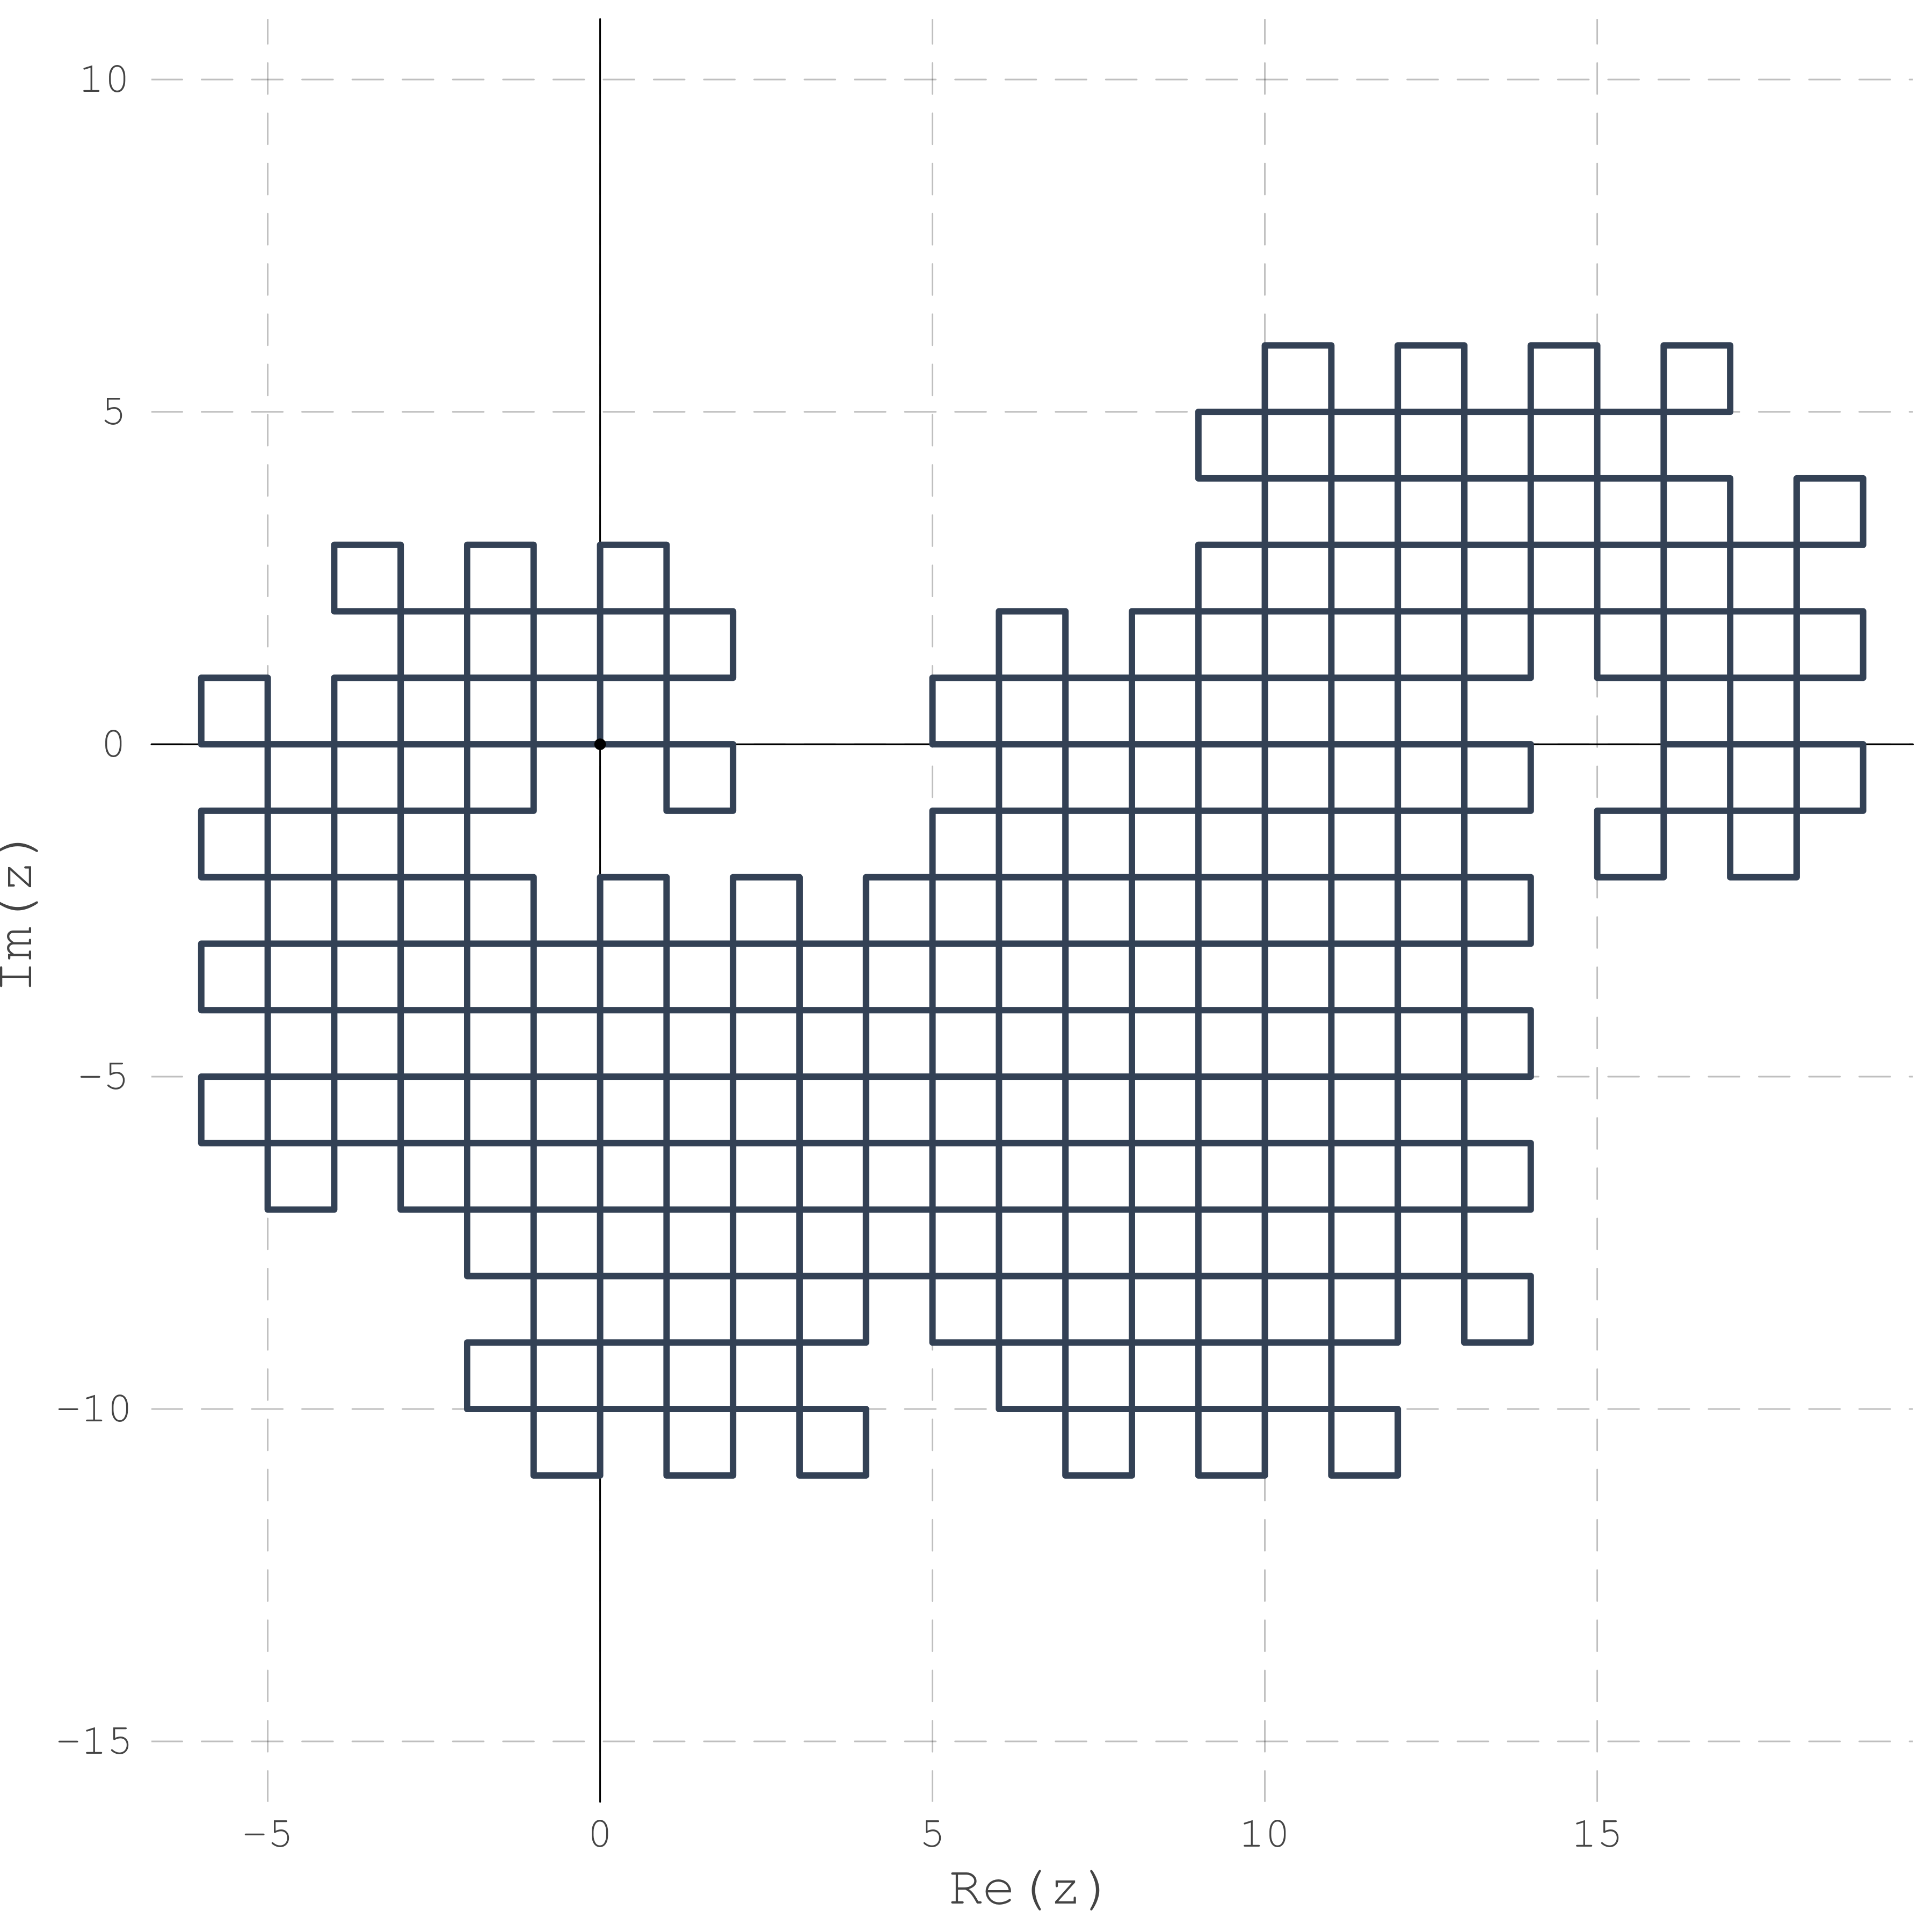
\includegraphics[width=0.46\linewidth]{assets/seed/curva_dragon_UDDDU_i8_p1.png}}
    
    \vspace{0.2cm} % Espacio vertical entre filas
    
    % Segunda fila
    \fcolorbox{gray!40}{white}{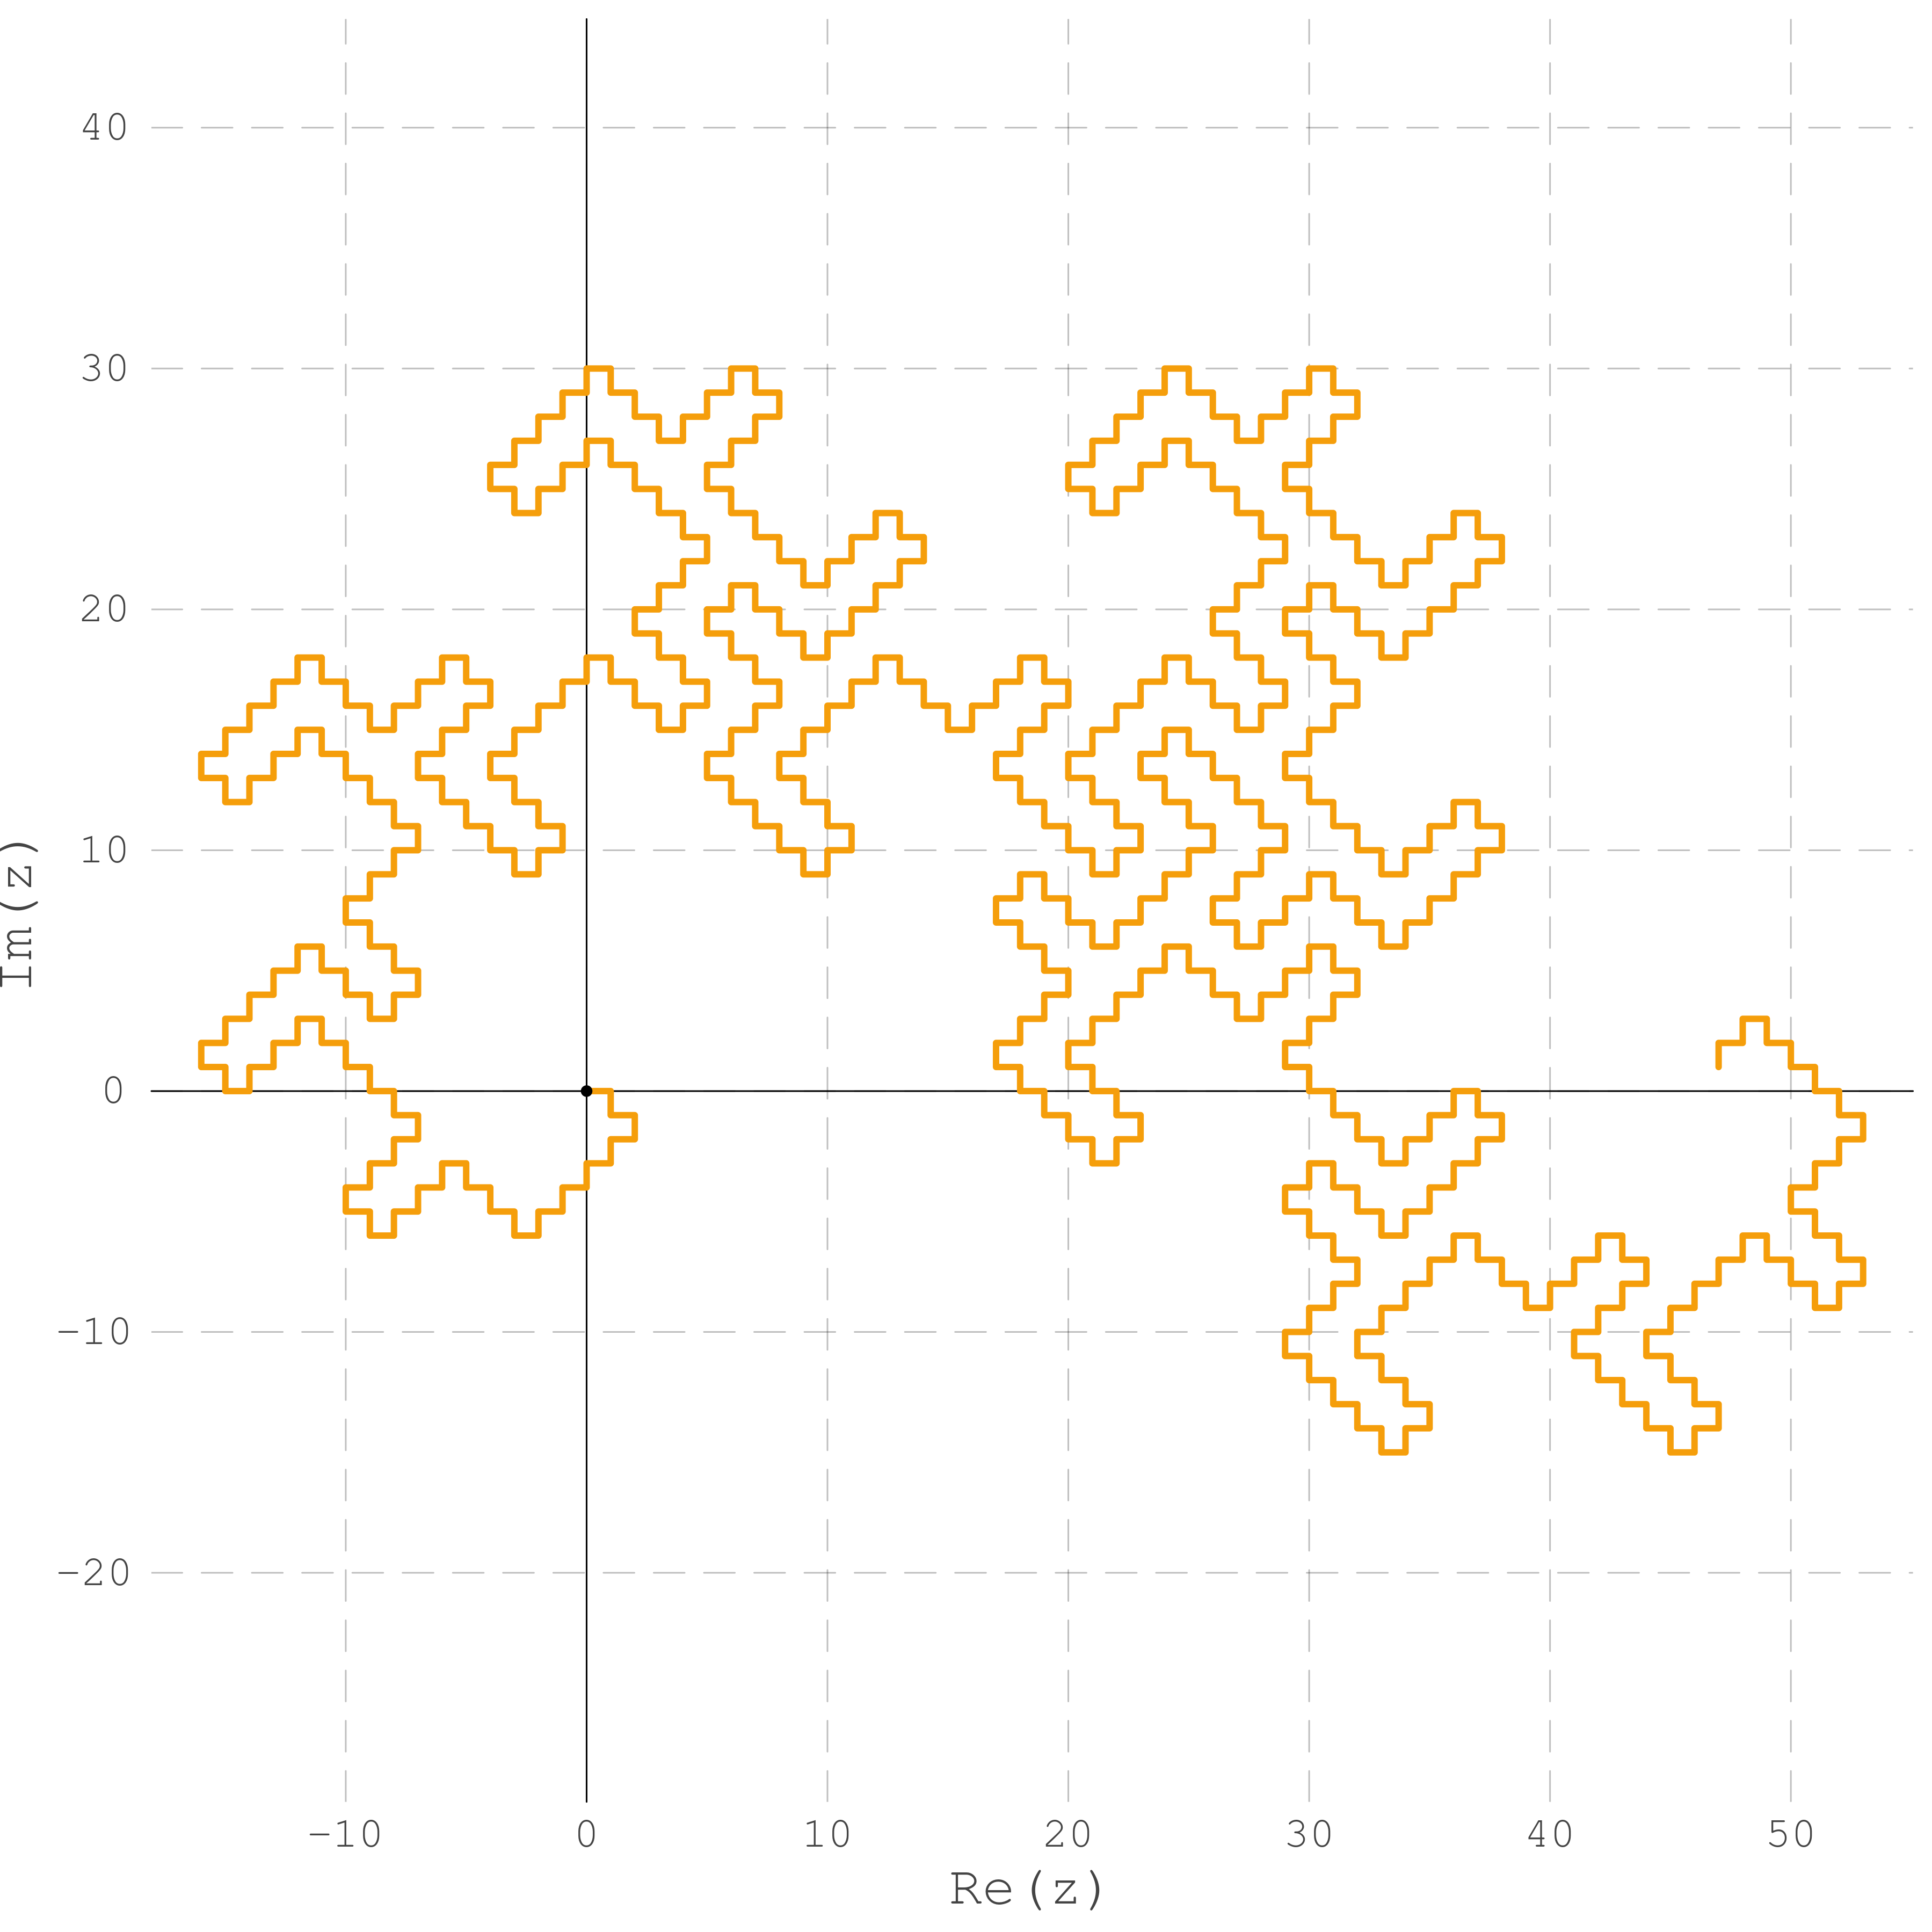
\includegraphics[width=0.46\linewidth]{assets/seed/curva_dragon_UDU_i8_p3.png}}\hspace{0.2cm}%
    \fcolorbox{gray!40}{white}{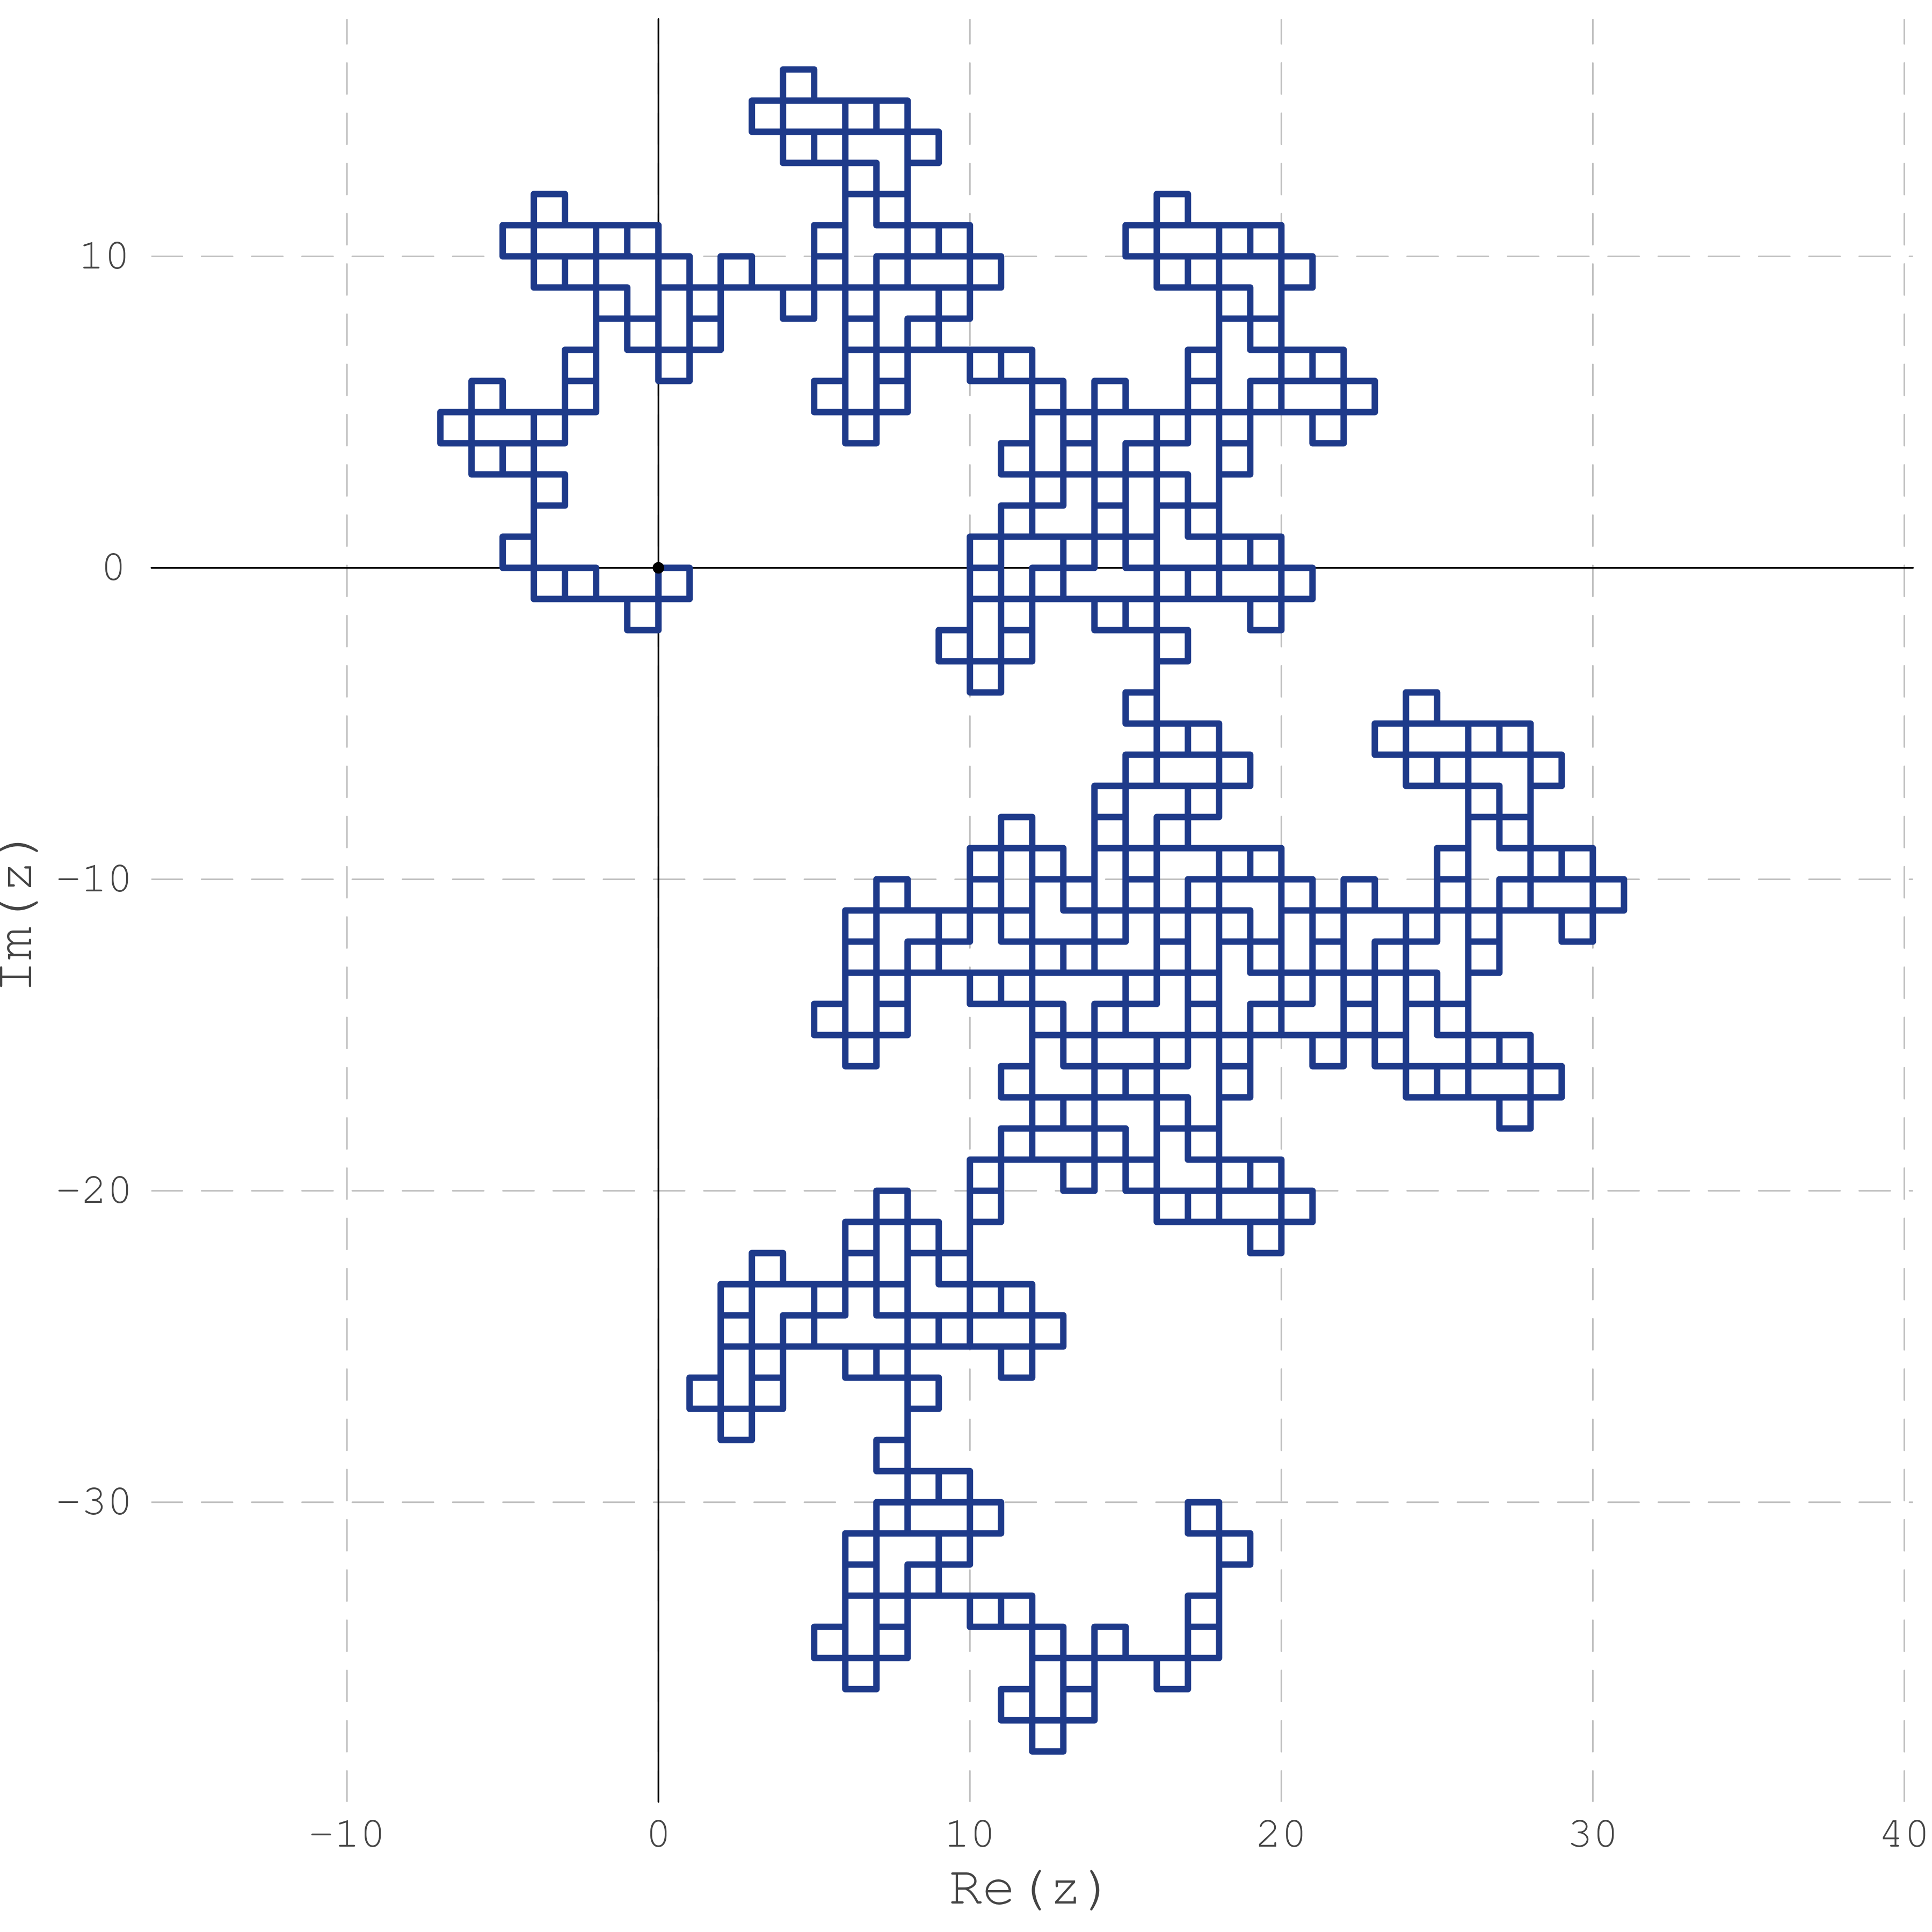
\includegraphics[width=0.46\linewidth]{assets/seed/curva_dragon_UUUUUUD_i8_p3.png}}
    
    \captionof{figure}{Dragones generados por las distintas semillas.}
    \label{fig:curva_dragon_semillas}
\end{center}
\end{defbox}
\begin{defbox}{Proposición. (Teselación del plano)}
Al tomar cuatro copias rotadas de la curva del dragón, es posible teselar el plano complejo, llenando el conjunto $\mathbb{Z}[i]$ de enteros gaussianos. 
\begin{center}
    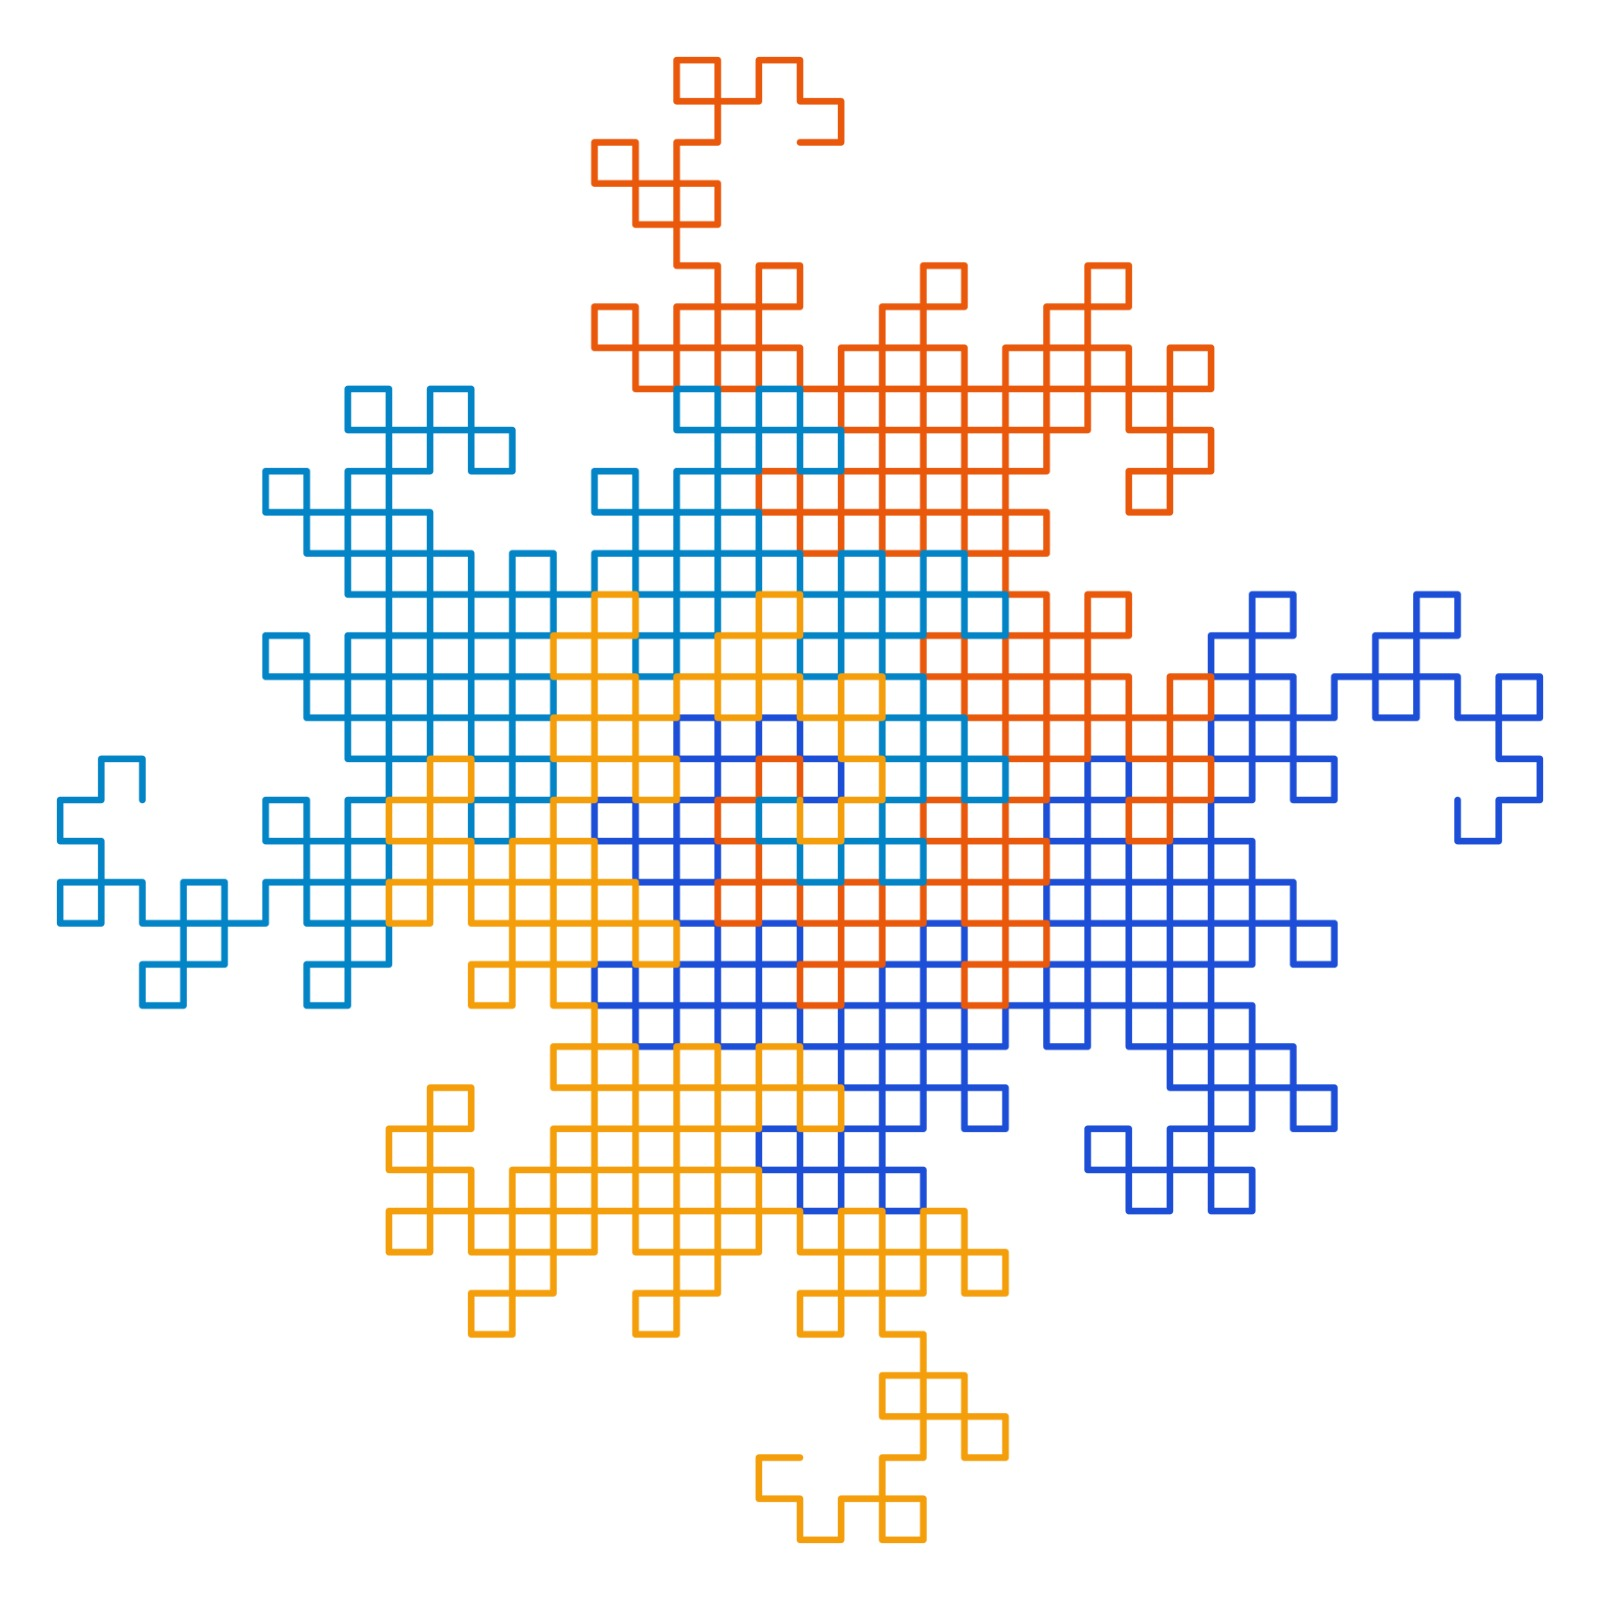
\includegraphics[width=1\linewidth]{assets/teselado/teselacion4colores.jpeg}
    \captionof{figure}{Cuatro dragones teselando el plano.}
    \label{fig:curva_dragon_teselando}
\end{center}
\end{defbox}

%%%%%%%%%%%%%%%%%%%%%%%%%%%%%%%%%%%%%%
\section{El dragón desde la teoría de categorías}
%Ahora se introducirán las herramientas categóricas para estudiar espacios \textit{autosimilares} siguiendo a \cite{Lei11}. 
El objetivo es encontrar soluciones de sistemas de ecuaciones en los que las variables representan espacios, cada uno igual al pegado de los demás \cite{Lei11}.
\begin{defbox}{Definición.}
Sea $G$ un endofuntor sobre una categoría $\mathcal{C}$. Una $G$\textbf{-coálgebra} es un par $(X,\xi)$ donde $X \in \mathcal{C}_\mathsf{o}$ es un objeto y $\xi: X \to G(X)$ es un morfismo en $\mathcal{C}$. Un morfismo de $G$-coálgebras $(X, \xi), (X', \xi')$ es un morfismo $f : X \to X'$ tal que $G(f) \circ \xi = \xi'\circ f$.
Un \textbf{punto fijo} de $G$ es una coálgebra $(X,\xi)$ donde $\xi$ es un isomorfismo.
\end{defbox}
Un espacio autosimilar se \textit{realiza} como un punto fijo de $G$.
\begin{defbox}{Lema de Lambek}
Si $(I, \iota)$ es terminal en la categoría de $G$-coálgebras, entonces $\iota : I \to G(I)$ es un isomorfismo.
\end{defbox}%Nos restringiremos al caso donde la categoría $\mathcal{C}$ es una categoría de diagramas sobre $\mathsf{Top}$. 
Un ejemplo importante es el caso del intervalo cerrado: se define la categoría cuyos objetos son espacios $X_1$ con dos \textit{extremos}; es decir, diagramas $X= (X_0, X_1, u, v)$ de la forma
\begin{center}
$X_0 \xrightarrow{\;u\;} X_1 \xleftarrow{\;v\;} X_0$
\end{center}
donde $X_0, X_1\in \mathsf{Top_o}$ y $u,v$ son inyecciones cerradas con imágenes disyuntas. Un morfismo $X \to X'$ consiste de dos funciones $f_0:X_0 \to X_0'$, $f_1: X_1 \to X_1'$ tales que $f_1 \circ u = u' \circ f_0$ y $f_1 \circ v = v'\circ f_0$.
El endofuntor $G$ se define pegando \textbf{dos copias de $X_1$ por un extremo}, mediante el pushout $X_1 \sqcup_{X_0} X_1$ del diagrama
\begin{center}
$X_1 \xleftarrow{\;u\;} X_0 \xrightarrow{\;v\;} X_1,$
\end{center}
identificando a $u(X_0)$ y $v(X_0)$ en las copias de $X_1$; esto es,
\begin{center}
    $G(X_0, X_1, u, v ) = (X_0, X_1 \sqcup_{X_0} X_1 , u', v')$.
\end{center}
Sobre esta categoría, considere el intervalo unitario
\begin{center}
$I = ( \{*\} , [0,1], u(*) = 0, v(*)= 1)$,
\end{center}
con el morfismo $\iota = (\iota_0 , \iota_1)$ dado por
\begin{align*}
    \iota_0 : \{*\} &\to \{*\} & \iota_1 : [0,1] &\to [0,2] \\
    * &\mapsto *, & t &\mapsto 2t.
\end{align*}
%$\iota = (\iota_0 :  \{*\} \to  \{*\}, \iota _1 : [0,1] \to [1,2])$, $\iota_0(*) = *$ y $\iota_1(t) = 2t$.
\begin{defbox}{Teorema (de Freyd - versión topológica).}
Para la categoría y el endofuntor $G$ definidos previamente, la $G$-coálgebra $(I, \iota)$ es terminal.
\end{defbox}
Este resultado caracteriza al intervalo unitario como un objeto que es homeomorfo a dos copias de sí mismo pegadas por un extremo, universal bajo esa propiedad.
%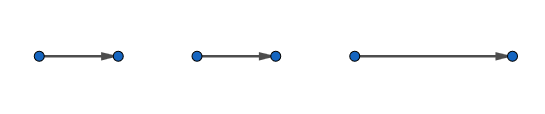
\includegraphics[width=0.5\linewidth]{assets/plegado/union segemntos.png}
Gracias a la definición recursiva de la palabra del dragón y su traducción geométrica como una curva en el plano, la construcción satisface la misma propiedad del intervalo cerrado: la curva es igual a dos copias homeomorfas de sí misma, pegadas por un extremo.
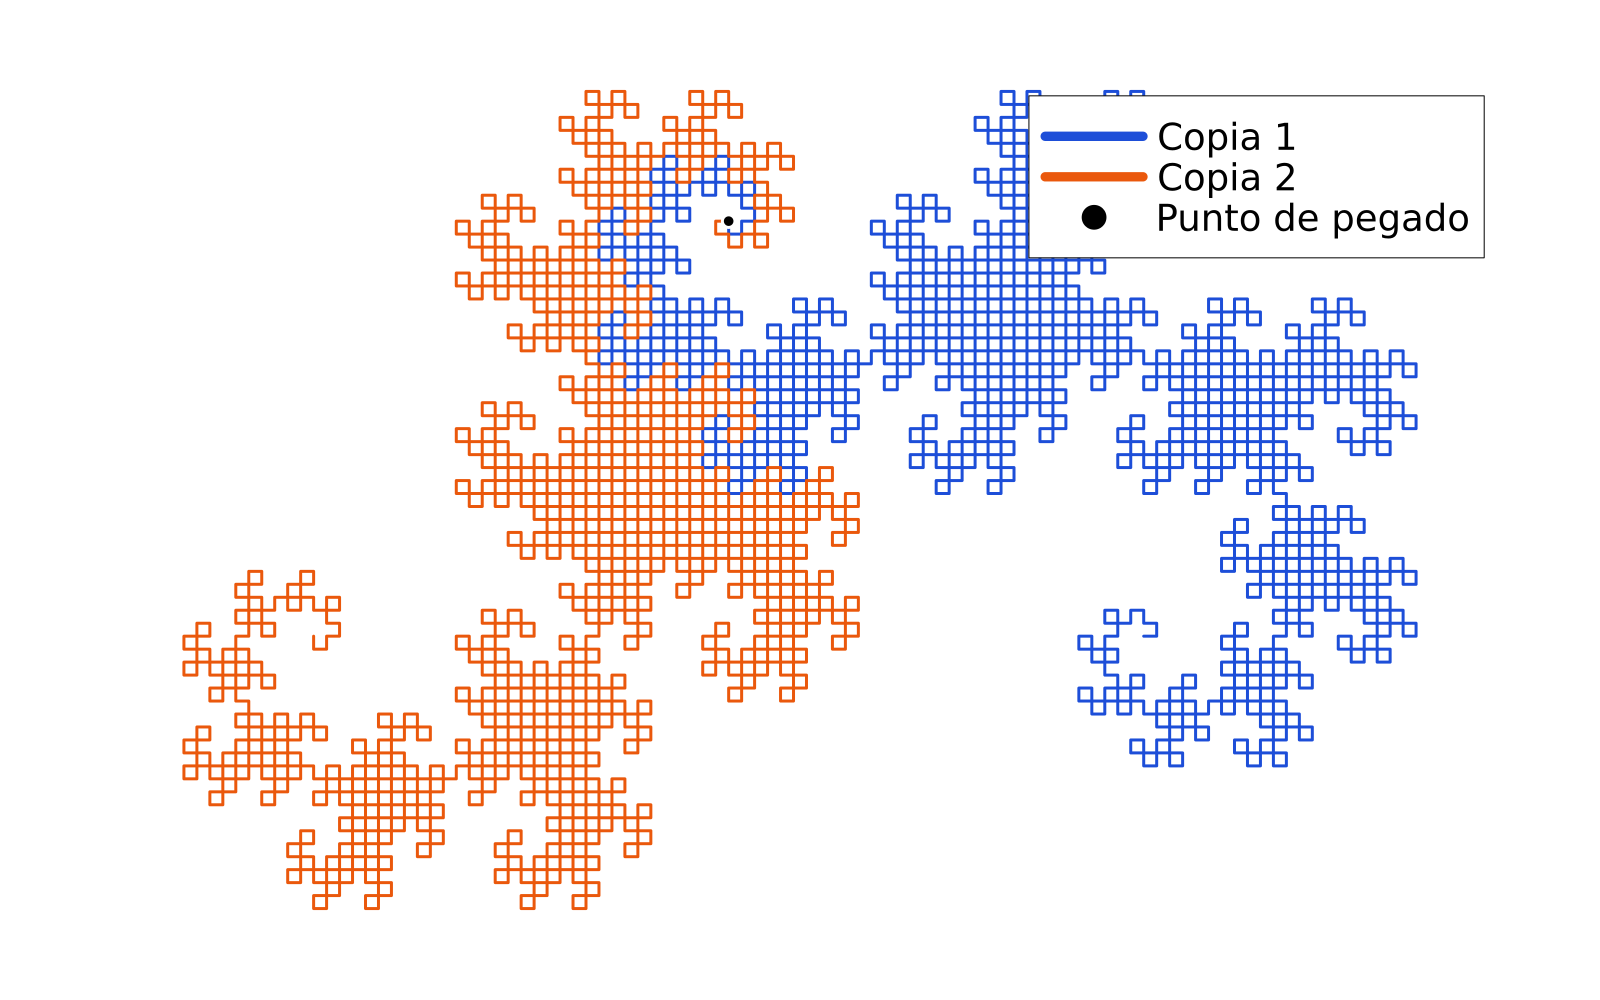
\includegraphics[width=1 \linewidth]{assets/plegado/dragon_autosemejante_i12.png}
\captionof{figure}{El dragón descompuesto en dos copias.}
Bajo la parametrización de la curva del dragón $D$ inducida por el sistema de plegado, la descomposición en dos copias de sí misma induce una estructura de $G$-coálgebra en $D$ que coincide con la del intervalo unitario. Por lo tanto, $D$ se realiza como punto fijo del funtor $G$; es decir, como solución universal del sistema autosimilar homeomorfo a dos copias de sí mismo, pegadas por un extremo.  
%%%%%%%%%%%%%%%%%%%%%%%%%%%%%%%%%%%%%%
\bibliography{biblio}

\end{multicols*}
\end{document}